\documentclass[crop,tikz,convert={density=300,size=1080x1080,outext=.png}]{standalone}
\usepackage{physics}
\usetikzlibrary{positioning}
\usetikzlibrary{arrows}

\begin{document}
%\begin{tikzpicture}[
%node/.style={shape=rectangle, minimum size=1.5cm, ,rounded corners=.2cm, draw=black, line width=1, fill=black!10},
%%edge/.style={-latex, thick},
%node distance=3cm,
%every text node part/.style={align=center}
%]
        %\node[rounded corners=.5cm, clip, inner sep=0] (obs) at (-8, 3) {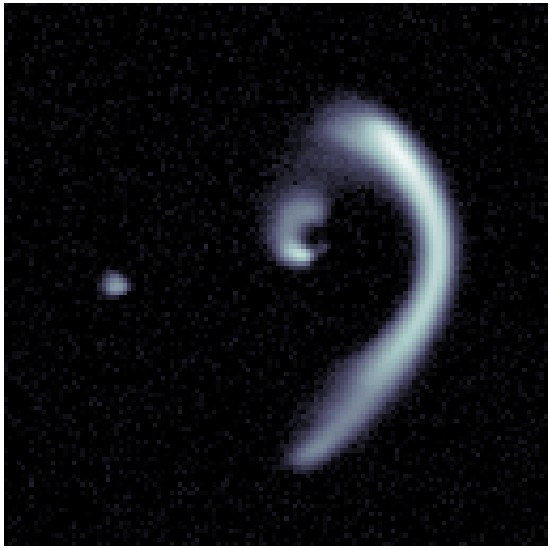
\includegraphics[width=2cm,height=2cm]{lens}};
        %\node[text=white] at (-8.6, 2.2) {$\mathbf{y}$};
        %\node[node, minimum width=4cm, minimum height=3cm] (x) at (1, 0) {};
        %\node at (2.5, 1.8) {$\mathbf{\hat{x}}^{(t)}$};
        %\node[rounded corners=.5cm, clip, inner sep=0] (source) at (2, 0) {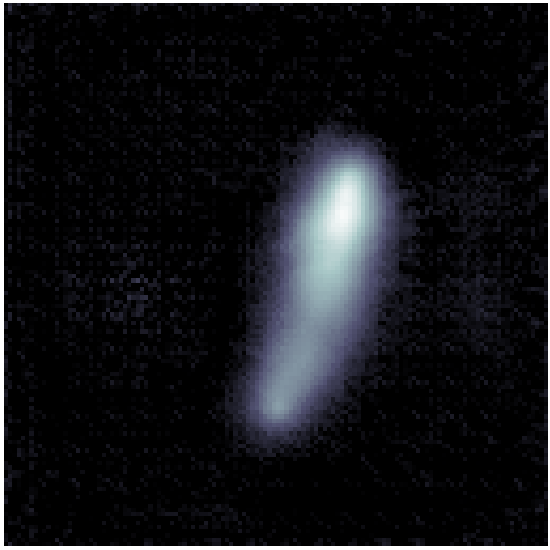
\includegraphics[width=2cm,height=2cm]{source_t2}};
        %\node[text=white] at (1.6, -0.7) {$\mathbf{\hat{s}}^{(t)}$};
        %\node[rounded corners=.5cm, clip, inner sep=0] (kappa) at (0, 0) {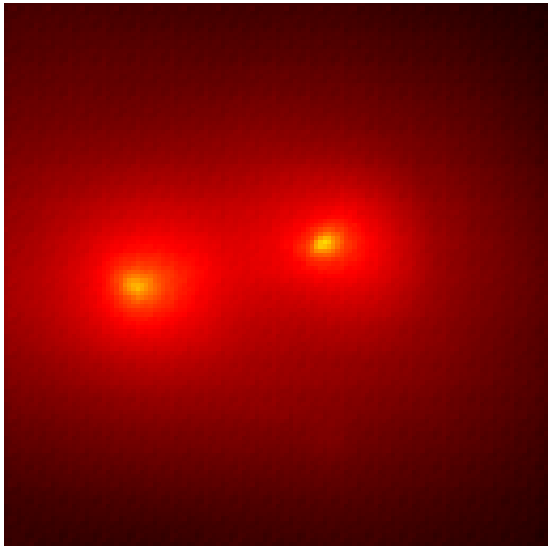
\includegraphics[width=2cm,height=2cm]{kappa_t2}};
        %\node[text=white] at (-0.4, -0.7) {$\boldsymbol{\hat{\kappa}}^{(t)}$};

        %\node[node] (F) at (1, -3) {Forward \\ Model};

        %\node[rounded corners=.5cm, clip, inner sep=0] (obs_pred) at (-4, -3) {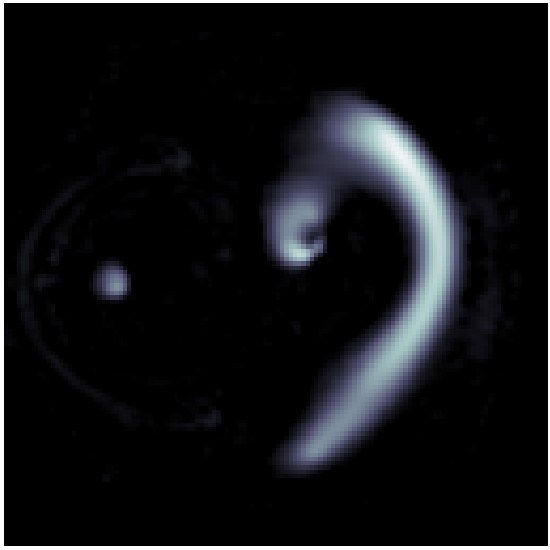
\includegraphics[width=2cm,height=2cm]{lens_t2}};
        %\node[text=white] at (-4.4, -3.7) {$\mathbf{\hat{y}}^{(t)}$};

        %\node[node] (rim) at (-4, 0) {Gradient \\ Update \\ $g_\varphi$};

        %%\node[node] (grad k) at (-8.7, -3) {$\displaystyle \frac{\partial \chi^2}{\partial \boldsymbol{\hat{\kappa}}^{(t)}}$};
        %%\node[node] (grad s) at (-7, -3) {$\displaystyle \frac{\partial \chi^2}{\partial \mathbf{\hat{s}}^{(t)}}$};
        %\node[node] (likelihood) at (-8, -3) {$p(\mathbf{y} \mid \mathbf{\hat{x}}^{(t)})$};

        %%\draw[-latex, thick, in=90, out=270] (source) to (F);
        %%\draw[-latex, thick, in=90, out=270] (kappa) to (F);
        %\draw[-latex, thick] (F) to (obs_pred);
        %\draw[-latex, thick] (rim) to (kappa);
        %\draw[-latex, thick] (obs_pred) to (likelihood);
        %\draw[-latex, thick] (obs) .. controls +(-1, -2) and +(-1, 2) .. (likelihood);
        %\draw[-latex, thick] (obs) .. controls +(0, -2.5) and +(-4, 0.5) .. (rim);
        %\draw[-latex, thick] (likelihood) .. controls +(0, 2.5) and +(-4, -0.5) .. (rim);
        %\node at (-7, -1) {$\grad_{\mathbf{y} \mid \mathbf{\hat{x}}^{(t)}}$};

        %\draw[-latex, thick] (x) to (F);

        %\draw[-latex, thick] (x) .. controls +(0, 3) and +(0, 3) .. (rim);

        %%\draw[-latex, thick] (obs_pred) to (grad s);
        %%\draw[-latex, thick] (grad s) .. controls +(0, 3) .. (rim);
        %%\draw[-latex, thick] (grad k) .. controls +(0, 4) .. (rim);

        %%\draw[-latex, thick] (source) .. controls +(0, 3) and +(-1, 3) .. (rim);
        %%\draw[-latex, thick] (kappa) .. controls +(0, 2) and +(0, 2) .. (rim);
\begin{tikzpicture}[
node/.style={shape=rectangle, minimum size=1.5cm, ,rounded corners=.2cm, draw=black, line width=1, fill=white},
every text node part/.style={align=center}
]
        \draw[draw=none] (-3, 4) rectangle (7, -4);
        %\node at (0, 3.3) {$\mathbf{\hat{x}}^{(t+1)} = \mathbf{\hat{x}}^{(t)} + g_\varphi (\mathbf{\hat{x}}^{(t)},\, \mathbf{y},\, \grad_{\mathbf{y} \mid \mathbf{\hat{x}}^{(t)}})$};

        \node[node, rounded corners=.2cm, minimum width=2cm, minimum height=2cm, fill=none, fill=black] (y) at (6, 3) {};
        \node[node, minimum width=4cm, minimum height=2cm, fill=none, rounded corners=.2cm, fill=black] (x) at (-1, 0) {};
        \node[rounded corners=.2cm, clip, inner sep=0] (obs) at (6, 3) {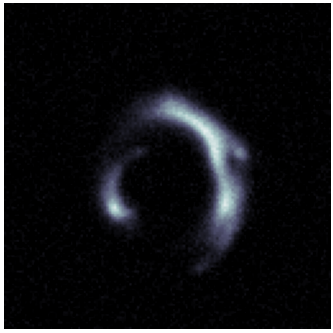
\includegraphics[width=2cm,height=2cm]{observation_highlight}};
        \node at (6, 4.2) {\Large $\mathbf{y}$};
        \node[color=white] at (6, 3.8) {Observation};
        \node[rounded corners=.2cm, clip, inner sep=0] (source) at (-2, 0) {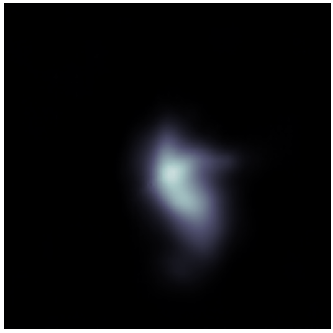
\includegraphics[width=2cm,height=2cm]{source_pred_highlight}};
        \node[color=white] at (-2, 0.8) {Source\strut};
        \node[rounded corners=.2cm, clip, inner sep=0] (kappa) at (0, 0) {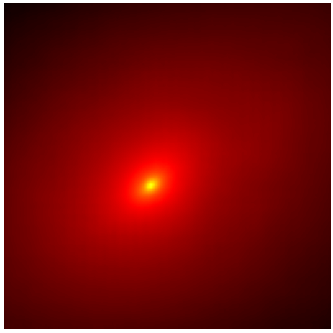
\includegraphics[width=2cm,height=2cm]{kappa_pred_highlight}};
        \node[color=white] at (0, 0.8) {Convergence};
        \node at (-2, 1.3) {\Large $\mathbf{\hat{x}}^{(t)}$};

        \node[node] (f) at (3, 0) {\LARGE $g_\varphi$};
        \draw[-latex, dashed, out=180, in=45, draw=black] (obs.west) to (f.north east);
        \draw[-latex, draw=black] (f.west) -- (kappa.east);

        \node[node] (F) at (-1, -2.5) {Raytracing};
        \draw[-latex, draw=black, dashed] (-1, -1) -- (F.north);

        \node[rounded corners=.2cm, clip, inner sep=0] (obs_pred) at (6, -2.5) {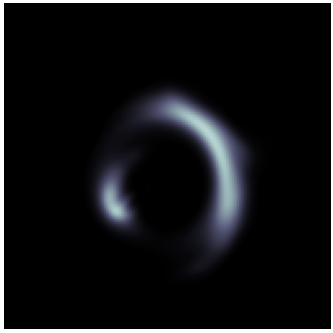
\includegraphics[width=2cm,height=2cm]{observation_pred_highlight}};
        \node[color=white] at (6, -1.8) {\scriptsize Reconstruction};
        \node[node, minimum width=2cm, minimum height=2cm, fill=none, draw=white] (y_pred) at (6, -2.5) {};
        \draw[-latex, color=black, dashed] (F) -- (y_pred);

        \node[node] (L) at (6, 0) {Likelihood};
        \draw[-latex, draw=black, dashed] (y_pred) -- (L);
        \draw[-latex, draw=black, dashed] (y) -- (L);

        \draw[-latex, color=black, dashed] (L) -- (f) node[midway, above] {$\grad_{\mathbf{y} \mid \mathbf{\hat{x}}^{(t)}}$};
        \draw[-latex, color=black, out=90, in=135] (-1, 1) to (f.north west);

\end{tikzpicture}
\end{document}
